% Selection rule: issue #145 nominated expanded-final/blocksworld-expanded-911101 (five blocks; goal on(b2,b4) and on(b3,b5) and on(b4,b3)). Each panel covers the relevant arms and observation types of this running task, showing the first decision where its illustrated behaviour occurs. Outcomes were inspected before this selection was finalised: these examples are illustrative, NOT pre-registered, and aggregate failure counts below supply context.
% Evidence Q1: outputs/expanded-study/v1/baseline/episodes/{visual,text}-state/expanded-final__blocksworld-expanded-911101/best_first_add_greedy-{process_sft,exact_reference}.json.gz events[].{input.current,input.successor_candidates,raw_output,view,successor_state} and result; outputs/expanded-study/v1/panel-v2/views/blocksworld-expanded-911101/scenes/catalog.json.gz states[].atoms and unlabelled/state-*.png. fig_qual_trace_solved.py asserts 18 decisions, 6 expansions, goal, identical text/visual raw outputs to reference, expanded h=(8,8,5,5,2,1), the s6 candidate rows and following s9. The cached 128px policy scenes are enlarged nearest-neighbour without re-rendering.
% Source discrepancy: the s6 stack(b4,b2) row has g=4, h=5, priority=5 and is closed/pruned; the figure-spec draft incorrectly gives g=5. The figure displays and asserts the actual cached episode's g=4.
\begin{figure}[tbp]
\centering
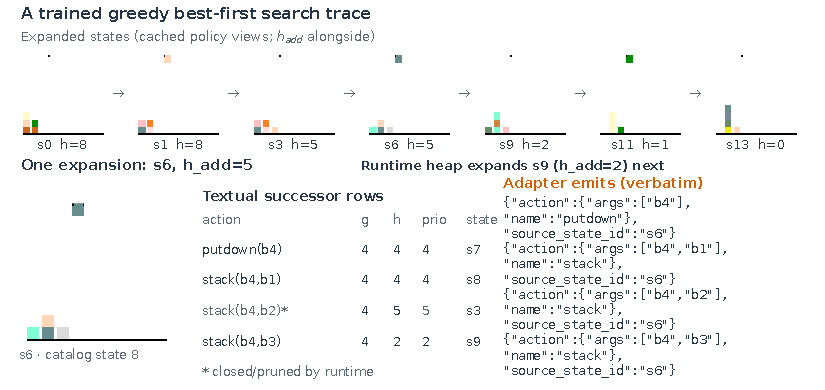
\includegraphics[width=\linewidth]{figures/fig_qual_trace_solved.pdf}
\caption{\textbf{A trained greedy best-first adapter reproduces the reference search on a five-block task.} Top: the six states the runtime expanded, with their $h_{\mathrm{add}}$, and the goal. Bottom: one expansion as the visual-observation adapter sees it, a rendered scene plus textual candidate rows with runtime-computed values, and the four operations it emits. Illustrative, not an efficacy estimate.}
\label{fig:qual-trace-solved}
\end{figure}

% Evidence Q2: outputs/expanded-study/v1/baseline/episodes/{text,visual,multimodal}-state/expanded-final__*/{bfs,best_first_width}-{process_sft,exact_reference}.json.gz events[].{input,raw_output,accepted,view}, result; bfs-random_valid.json.gz (145-decision cap); docs/experiments/expanded-study/failure-mechanism-tables/failures-by-cell.csv (24 BFWS malformed outputs per observation type; BFS bookkeeping/frontier categories). fig_qual_trace_failures.py recomputes all 24 x 3 main-grid episodes: BFS 68 successor failures (67 unvisited and 1 revisited) plus 4 premature retire_frontier; BFWS 72 decision-0 failures (32 unparseable, 40 parseable with invented keys, 17 naming the reference action). CSV BFS strata have 27, not 24 episodes per observation type, so their extra three are excluded from those main-grid counts; their presumed DAgger origin is not verified. The shown b1-held scene is the cached unlabelled/state-000001.png.
% Q2 training-count evidence: outputs/matched_modalities/{v3,v5}/training/{text,visual,multimodal}-state/{bfs,best_first_width}/report.json train_records and training_record_ids, matched to each baseline episode's checkpoint; fig_qual_trace_failures.py asserts 512 records for all six shown learned cells. BFS candidate statuses follow accepted exact-reference successors and their catalog state atoms, with stack(b1,b4) restoring the already visited initial state.
\begin{figure}[tbp]
\centering
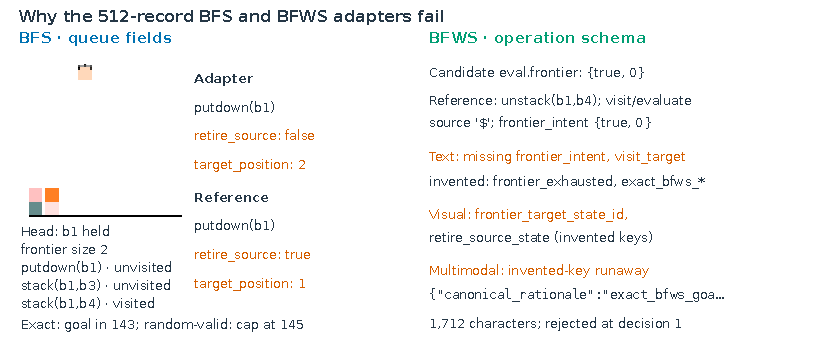
\includegraphics[width=\linewidth]{figures/fig_qual_trace_failures.pdf}
\caption{\textbf{At 512 records, BFS fails on queue bookkeeping and BFWS on the operation format.} Left: the BFS adapter names a valid successor but misstates whether the head is retired and the queue position (differences in orange); all three observation types give this error. Right: the BFWS adapter names the reference action but writes a malformed operation.}
\label{fig:qual-trace-failures}
\end{figure}

% Evidence Q3: outputs/expanded-study/v1/modality-stress/episodes/{text,multimodal,visual}-state/expanded-final__blocksworld-expanded-911101/best_first_add_greedy-{text-shuffled,visual-blank,visual-degraded}-learned_adapter.json.gz events[].{input,raw_output,accepted,view}, result and checkpoint; baseline/episodes/{text,visual,multimodal}-state/.../best_first_add_greedy-process_sft.json.gz checkpoint; configs/experiments/expanded-study/modality-stress-protocol.json corruption_master_seed=42613; examples/planning_benchmark_slice/expanded_modality_stress.py _corrupt_image; panel-v2/views/blocksworld-expanded-911101/unlabelled/state-000000.png. fig_qual_trace_corruption.py asserts same main-grid checkpoint, rejected shuffled outputs at decisions 2/3 and 18-decision success for all four visual-blank/degraded runs. Blanking/degradation follows the frozen PIL recipe; no unverified shuffled-text excerpt is shown.
\begin{figure}[tbp]
\centering
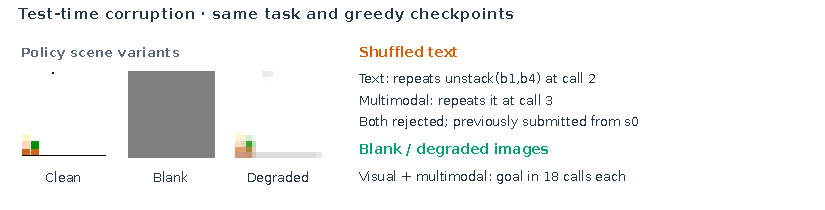
\includegraphics[width=\linewidth]{figures/fig_qual_trace_corruption.pdf}
\caption{\textbf{The same greedy adapters fail when their text is shuffled and solve with blanked or degraded images.} With shuffled text, the text and multimodal adapters resubmit an operation they already submitted and are rejected at decisions 2 and 3. With blanked or degraded images, the visual and multimodal adapters solve the task in 18 decisions.}
\label{fig:qual-trace-corruption}
\end{figure}
